\chapter{Referencial Teórico}
\label{chap:Ref}
	Neste capítulo serão apresentados os conceitos utilizados na pesquisa, bem como
	os estudos que fundamentaram esse projeto. A \cref{sec:Mooc} apresenta
	o conceito de \acs{MOOC} e as principais características da plataforma de ensino.
	A \cref{sec:FundTeor} descreve as os principais conceitos relacionados à
	mineração e visualização: mineração, visualização, projeção, agrupamento e
	classificador. A \cref{sec:MinVisual} descreve as características que
	podem ser extraídas dado a escolha de um dos tipos de análise de código-fonte.
	Finalmente, a \cref{sec:TrabRel} apresenta as pesquisas relacionadas a este estudo
	juntamente com suas limitações.

	\section{Massive Open Online Courses (MOOC)}
	\label{sec:Mooc}
		Após pesquisar o conceito de Curso Massivo, Aberto e \foreign{Online},
		\citeonline{fassbinder2014} observam que não há uma definição comum na
		literatura. Encontram-se três descrições distintas para o termo.
		\citeonline{sivamuni2013} afirmam que o \acs{MOOC}, em conformidade com o
		dicionário Oxford, é um curso oferecido por meio da Internet, de forma
		gratuita, para uma grande quantidade de alunos. \citeonline{subbian2013}
		reitera que o \acs{MOOC} disponibiliza curso gratuito, baseado na \foreign{web},
		com registro livre de taxas monetárias e compartilhamento público de
		currículo. Por fim, \citeonline{siemens2013} defende a tendência em inovação e
		experimentação do uso da tecnologia para o ensino a distância e
		\foreign{online} a fim de dar oportunidade de aprendizagem de forma massiva.
		Não obstante, observa-se a concordância quanto ao oferecimento pela Internet
		e para grande quantidade de pessoas (massivo).
		
		\citeonline{kim2014} afirmam que massivo refere-se a capacidade do \acs{MOOC} em
		suportar uma grande quantidade de alunos. Tal quantidade é bem superior
		ao número de discentes que uma sala pode acomodar ou o total de
		participantes em um curso \foreign{online} antes do surgimento do \acs{MOOC}.
		Por exemplo, um curso de Inteligência Artificial foi ofertado, \foreign{online}
		e gratuitamente, pela Universidade de Stanford em 2011, no qual houveram
		160.000 estudantes inscritos \cite{rodriguez2012}.
		
		Os principais recursos das plataformas utilizados para \acs{MOOC} são a integração
		com outras aplicações, como a utilização de e-mails e fóruns, o uso de questionário
		relacionados com os vídeos e a inclusão de atividades para estimular e motivar
		os alunos \cite{fassbinder2014}. Os fóruns de discussão auxiliam os usuários
		a aprenderem sobre o problema abordado \citeonline{schmidt2013producing}.
		Em adição, também é possível utilizar recursos para avaliar alguns tipos de
		teste, como as questões de múltipla escolha, na qual verifica-se a alternativa
		selecionada com a presente no gabarito de questões \citeonline{alario2013analysing}.
		% TODO: acrescentar algo  quanto a integração, voltado a integração de aplicação para auxiliar na avaliação de tarefas. Citar trabalhos/pesquisas sobre a integração desse tipo de instrumentos/aplicações em MOOC (tanto os que citamos na seção de mineração e visualização e que usam dados de MOOC quanto outros de avaliação como um todo). Daí sim siga com o texto que "Focaremos no desenvolvimento...".
		Focaremos no desenvolvimento de recursos avançados de visualização dos dados
		obtidos por meio das implementações submetidas em cursos de programação e na
		realização de \foreign{feedback} para que o usuário possa verificar seu
		nível de conhecimento.

	\section{Mineração e Visualização de Dados}
	\label{sec:FundTeor}
		Nesta seção apresentaremos as definições de alguns termos utilizados
		durante a pesquisa: mineração, a diferença na área de Inteligência
		Artificial sobre classificadores e agrupamento, visualização de dados e projeção.

		\begin{figure}[h]
			\centering
			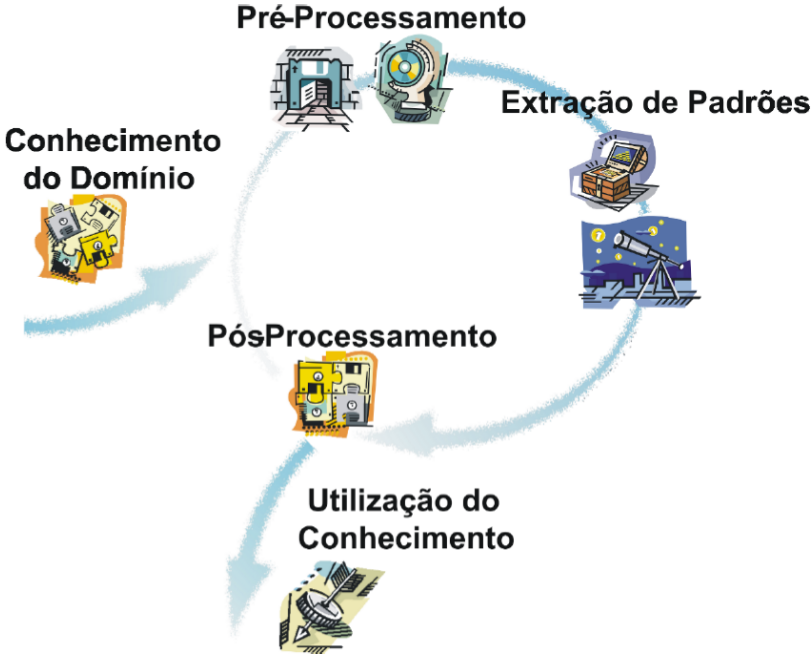
\includegraphics[width=0.6\linewidth]{imagem/mineracaoDados}
			\caption[Etapas da mineração de dados]{Etapas da mineração de dados \cite{rezende2003}}
			\label{fig:mineracaoDados}
		\end{figure}
		
		A mineração de dados é uma etapa do \foreign{Knowledge Discovery in Databases}
		\cite{fayyad1996} que busca descobrir padrões em grandes conjuntos de dados,
		podendo utilizar métodos de inteligência artificial, estatísticos e sistemas
		de banco de dados \cite{chakrabarti2006}. O objeto do processo de mineração
		de dados consiste na extração de informações de um conjunto de dados e
		transformá-lo em uma estrutura compreensível para uso posterior \cite{chakrabarti2006}.
		A \cref{fig:mineracaoDados} apresenta os estágios da mineração de dados:
		o Conhecimento do Domínio condiz com a identificação do problema para possuir
		um conhecimento inicial e definir as metas e os objetivos a serem atingidos
		no processo de extração de conhecimento; a etapa Pré-processamento refere-se
		a padronização e limpeza de dados extraídos de fontes diversas e  a escolha
		de um subconjunto representativo; a fase seguinte, Extração de Padrões, 
		consiste na aplicação do algoritmo de mineração de dados escolhido; o estágio
		Pós-processamento equivale a análise dos padrões obtidos anteriormente e
		possibilita a extração de outros padrões; por fim, a Utilização do Conhecimento
		é a utilização dos dados extraídos em algum sistema ou utilizado diretamente
		pelo usuário. Observe que esse sistema pode se realimentar, caso seja necessário
		adicionar mais informações, dessa forma, necessita-se realizar essas etapas
		novamente realimentando o sistema com novas características. % TODO: faltou completar algo aqui... se realimentar de que e onde?
		
		Muitos métodos de mineração de dados são baseados em técnicas de treinamento
		e teste de aprendizagem de máquina e, reconhecimento de padrões e estatísticas,
		como os algoritmos de classificação e agrupamentos, respectivamente \cite{fayyad1996}.
		
		Classificação é a tarefa de aprendizagem de uma função alvo que mapeia cada
		conjunto de atributos a um dos rótulos de classe predefinidas \cite{Tan:2005:ch4}.
		Uma função alvo auxilia uma ferramenta, que possui informações, a distinguir
		os objetos de diferentes classes. A fim de realizar essas classificações, são
		implementados classificadores com diversas abordagens, como árvores de decisão,
		redes neurais e \foreign{support vector machine}, por exemplo. Esses
		classificadores são mais utilizados para predizer ou descrever um conjunto
		de dados com categorias binárias ou nominais \cite{Tan:2005:ch4}. Por exemplo,
		para classificar um animal como mamífero, réptil, peixe, anfíbio ou pássaro,
		deve-se sumarizar dados como a temperatura do corpo, característica da pele,
		se é uma criatura aquática, se possui patas e hiberna.
		
		O que difere a classificação do agrupamento é que esse é formado por meio da
		comparação de informações entre os objetos e não existem rótulos pré-definidos,
		enquanto aquele é realizado por meio da comparação das informações do objeto
		com os dados contidos em cada classe predefinida da função alvo. Desta forma,
		os objetos dentro de um grupo devem ser similares ou relacionados entre si e
		diferentes ou não relacionados entre objetos de grupos diferentes, ou seja,
		quanto maior a similaridade dos objetos dentro de um grupo e mais diferentes
		são os agrupamentos, melhor ou mais distinto os agrupamentos \cite{Tan:2005:ch8}.
		O K-means \cite{macqueen1967} e o \ac{DBSCAN} \cite{Ester1996} são exemplos de
		algoritmos de agrupamento.

		Após a mineração dos dados, é desejável a utilização de ferramentas para
		auxiliar na criação de hipóteses sobre conjuntos de dados complexos -- grande
		conjunto de dados ou de alta dimensionalidade -- para que os analistas possuam
		capacidade de explorá-los e compreendê-los \cite{de2003}. A visualização de dados
		produz modelos gráficos e representações visuais a fim de utilizar a capacidade
		cognitiva do ser humano, por meio da percepção visual, para colaborar com
		a exploração e obtenção de informações úteis presente nos dados \cite{de2003,keim2002}.
		Ademais, a visualização de dados é intuitiva, permitindo explorar os dados
		mais rápido e fornecendo melhores resultados na maioria das vezes \cite{keim2002}.
		
		Entretanto, não é possível gerar visualizações sobre conjuntos de dados
		complexos. Assim sendo, é necessário a utilização de técnicas de projeção que
		criam o mapeamento de dados para reconhecimento visual \cite{friedman1974} e,
		com isso, produzir a visualização. Devido a alta dimensionalidade dos dados,
		é necessário a utilização de projeções multidimensionais. Essa técnica realiza
		a diminuição n-dimensional, sendo $n$ uma alta dimensão, para uma espaço
		unidimensional, bidimensional ou tridimensional \cite{paulovich2008least},
		sempre buscando a menor perca de informação possível, como a relação de
		similaridade do espaço n-dimensional no espaço unidimensional, bidimensional
		ou tridimensional. Para criar essa visualização deve-se selecionar o formato
		de como as características extraídas serão armazenadas, como o vetor de
		características ou o modelo de tabela de dados \cite{de2003}.
		
		\subsection{Dissimilaridade de dados}
		Dianta da necessidade de uma medida conter quatro propriedades - não-negatividade,
		identidade, simetria e desigualdade triangular - para que possa ser considerada
		uma métrica, há medidas que não obedecem a essas propriedades, mas que também
		são importantes, conhecido como dissimilaridade \cite{phd:paulovich}. Tais
		dissimilaridades produz um grupo maior de medidads, já que pode conter qualquer
		tipo de função que compare numéricamente o quanto dois objetos podem ser
		diferentes \cite{Tan:2005:IDM:1095618}.
		
		Considerando espaços de alta dimensão e esparsos, é preferível a utilização
		da inversão da similaridade do cosseno, visto que comparações entre zeros
		não afeta seu resultado. Isso é consequência da dependencia do número
		de medidas que os objetos compartilham entre si, suprimindo os números
		não existentes entre eles \cite{phd:paulovich}. Nesse caso de alta
		dimensionalidade dos dados e esparços, essa aspecto torna-se desejável pelo
		fato da limitação do conjunto de características com medidas diferentes de
		0 (zero), com isso serão correspondentes por meio das características que não
		os representa, iguais a 0 (zero) \cite{Tan:2005:IDM:1095618}.
		
		\citeonline{phd:paulovich} afirma que há dois cenários distintos que podem
		adulterar o resultado: quando a norma Euclidiana do vetor de característica
		que representa os objetos são muito diferentes; e quando alguns aspectos
		do vetor de características possuem valores em escalas diferentes dos demais
		atributos do vetor. Tais cenários podem ser evitados. Para evitar a primeira
		situação, aplica-se o processo de normalização para que todos os vetores possuem
		norma Euclidiana unitária. Enquanto a segunda situação evita-se por meio da
		aplicação de um processo chamado padronização (\foreignlanguage{standardization})
		\cite{Tan:2005:IDM:1095618}, atribuindo novos valores com média igual a 0 (zero)
		e desvio padrão igual a 1 (um), por meio da transformação da média de cada
		característica com seu desvio padrão.
		
		%TODO
		Professora Aretha, na página 15 da tese do Paulovich, no seguinte parágrafo:
		"Para evitar o primeiro cenário um processo de normalização...". Ele fala sobre
		a média da COORDENADA. Eu não entendi se essa média é daquela característica
		específica ou do vetor de característica, apesar de ter escrito:
		"por meio da transformação da média de cada característica com seu desvio padrão."

	\section{Mineração e Visualização de Programas}
	\label{sec:MinVisual}
		Para realizar a mineração de informações nos programas submetidos, é necessário
		decidir como serão extraídos as características -- análise sintática, dinâmica e
		do código de escrita -- e quais dados podem ser obtidos por meio da análise
		escolhida (\cref{subSec:Caracteristicas}). Independente da dimensão
		obtida por meio da quantidade de informações extraídas, é necessário escolher
		como os dados obtidos serão representados para que seja possível realizar sua visualização.
		
		\subsection{Características de Programas}
		\label{subSec:Caracteristicas}
		
			\begin{figure}[h]
				\centering
				\includegraphics[width=0.7\linewidth]{imagem/fluxoProgramacao}
				\caption{Representação da implementação de um problema}
				\label{fig:fluxoProgramacao}
			\end{figure}
			
			Um programa de computador é um conjunto de instruções computacionais que visa
			solucionar um problema. A \cref{fig:fluxoProgramacao} apresenta os passos
			necessários para que um programa exista. O primeiro passo consiste na
			identificação do problema a ser solucionado. Por exemplo, um fila indiana
			criada aleatoriamente, no qual não é possível visualizar todos os participantes
			presentes nessa fila. Em seguida, deve-se elaborar um algoritmo para que seja
			possível resolver esse problema. O algoritmo é constituído por uma sequência
			de passos que resolva algum problema, condizendo com o que deve ser feito.
			Por fim, realiza-se a implementação do algoritmo, definindo como as instruções
			devem ser executadas.

			A extração de características por meio das implementações pode ocorrer das
			seguintes formas: análise estática, análise do estilo de escrita e análise dinâmica.
			A análise estática ocorre por meio da observação do código-fonte, considerando
			apenas sua implementação, ou seja, não é necessária sua execução. Há diversas
			características que podem ser extraídas dessa análise. Há abordagens que extraem
			somente a \ac{AST} que pode ser gerada durante a análise
			sintática do compilador para representar o código-fonte em forma de árvore
			armazenando símbolos não-terminais nos nós filhos e símbolos terminais nos
			nós folha, como representa a \cref{fig:AST} em uma declaração de condição.
			Esse tipo de árvore possui símbolos não terminais como nós filhos
			e símbolos terminais como nós folhas. Enquanto outras abordagens extraem
			características como: a quantidade de linhas e atribuições da implementação,
			a complexidade ciclomática \cite{mccabe}, quantidade de variáveis, operadores,
			operandos, laços de repetição e laços de repetição aninhados, por exemplo.
						
			\begin{figure}[h]
				\centering
				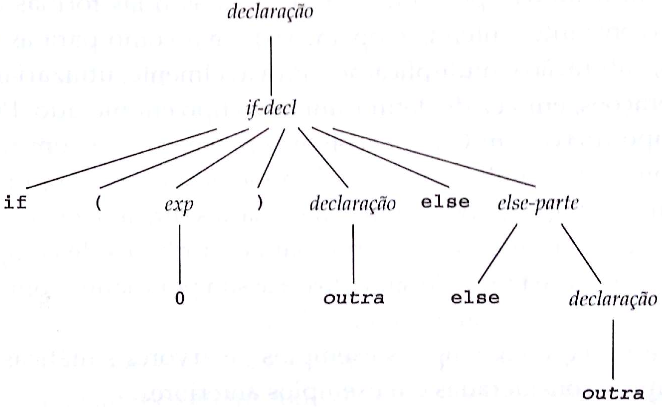
\includegraphics[width=0.7\linewidth]{imagem/AST}
				\caption[Representação de árvore de sintaxe abstrata]{Representação de árvore de sintaxe abstrata \cite{louden2004}.}
				\label{fig:AST}
			\end{figure}
			
			A análise do estilo de escrita é um tipo da análise estática. Entretanto,
			se difere no fato das implementações estarem sintaticamente corretas. Nesse
			tipo de análise é considerado o estilo de escrita do programador, abrindo a
			possibilidade de coletar dados como: indentação, há mais que uma instrução e importação
			de bibliotecas por linha, há espaços entre operando e operador, os métodos
			são separados por uma linha em branco, tamanho da instrução  medido em
			caracteres e espaço entre operando e operador, por exemplo (\cref{apendice:pep8}).
			A \cref{tab:exemploEstEsc} exemplifica possíveis características
			extraídas em uma chamada de função, na qual é possível inserir ou não um
			espaço entre o parâmetro e os \foreign{tokens} abrir e fechar parêntese,
			como também a utilização de uma ou mais instruções por linha. Caso a primeira
			chamada de função e as duas primeiras instruções separadas por uma quebra de linha
			forem o padrão para o estilo de escrita, sua ocorrência não gerará nenhum
			aviso. Contudo, caso ocorra as outras três chamadas de função, os quais
			possuem espaços em branco, ou mais de uma instrução por linha separados
			por \texttt{;} (ponto e vírgula), é informado um tipo de erro.
			
			\begin{table}
				\centering
				\begin{tabular}{|c|c|}
					\hline
					Chamada de função & Instrução por linha \\ \hline
					primo(7)		  & a = 5 * 3  \\
					primo( 7)		 & primo(7)	 \\
					primo(7 )		 &	  \\
					primo( 7 )		& a = 5 * 3; primo(7)	\\
					\hline
				\end{tabular}
				\caption[Representação do estilo de escrita]{Representação do estilo
				de escrita em uma chamada de função e instrução por linha.}
				\label{tab:exemploEstEsc}
			\end{table}
			
			A análise dinâmica do código-fonte consiste na observação da execução do
			programa, por meio do rastro de execução
			do programa (\foreign{trace}) e de teste de \foreign{software}. Analisando esse histórico é
			possível verificar algumas características, como: em que momento foi realizado
			uma atribuição, chamada de função e recursão, qual bloco de código foi
			executado em uma declaração de condição, a quantidade de vezes que um laço
			de repetição foi executado e a saída no final da execução. Já o teste de
			software pode ser utilizado executando casos de teste nos quais é verificado
			se produção final do programa era o esperado e esta informação, se o caso de
			teste funcionou corretamente ou não, também pode ser uma característica do programa.
			
			Além da possibilidade de extrair os dados citados anteriormente, é possível
			obter os dados de como foi realizado o processo técnico e social do desenvolvimento
			do programa. Para ambas abordagens, é necessário a utilização de um sistema de
			controle de versão para que se possa utilizar seus recursos. Um mecanismo para
			obter informações é em relação ao momento, data e hora em que o aluno realizou
			um \foreign{commit} de uma versão da sua implementação. Outro método é verificar
			se houve comunicações com outras pessoas durante o desenvolvimento do programa,
			por meio da interação em \foreign{issues} ou solicitações de \foreign{pull requests}.
			
			O programa é a implementação do algoritmo que soluciona um problema e é realizado
			mediante seu entendimento. O problema, por sua vez, pode exigir conhecimento e
			uso de técnicas de programação específicas, a utilização de laço de repetição,
			por exemplo. 

<<<<<<< HEAD
	\subsection{Mineração e visualização}
=======
	\section{Trabalhos Relacionados}
>>>>>>> d80c3a12312ba77213ace652eb951e0fce85b640
	\label{sec:TrabRel}
	
		A fim de encontrar a semelhança entre os códigos, \citeonline{Yin:2015}
		utilizaram a AST dos programas submetidos pelos alunos. Após a criação das
		árvores, é necessário o uso de métricas para verificar a similaridade entre
		as árvores. Desta forma, foi utilizada a Distância de Edição de Árvore (\ac{TED})
		– ao comparar duas árvores, verificam-se quais são as movimentações (inserção,
		movimentação e remoção) necessárias para que as árvores fiquem iguais. Mais
		precisamente, foi selecionada a \acs{TED} normalizada, atribuindo pesos maiores para
		os nós mais próximos da raiz (de menor altura) \cite{zhang1989simple}, quanto
		mais próximo do nó raiz, maior sua importância.

		A \acs{TED} normalizada realiza comparações nó a nó da raiz até as folhas, priorizando
		os nós mais próximos da raiz, atribuindo um peso maior a eles. A fim de evitar
		que pequenas diferenças na sintaxe influenciem diretamente na pontuação de
		similaridade, visto que a estrutura podem ser semelhantes, diferenciando-os
		em detalhes de baixo nível.
		
		Os autores desse artigo utilizaram o algoritmo de agrupamento \ac{OPTICS}
		\cite{Ankerst1999} para agrupar os códigos semelhantes. Para visualizar os
		agrupamentos foi utilizado o \ac{t-SNE} \cite{maaten2008} – técnica utilizada para
		reduzir dados de alta dimensionalidade para duas ou três dimensões preservando
		a estrutura local dos dados.
		
		
		\begin{figure}[h]
		\centering
		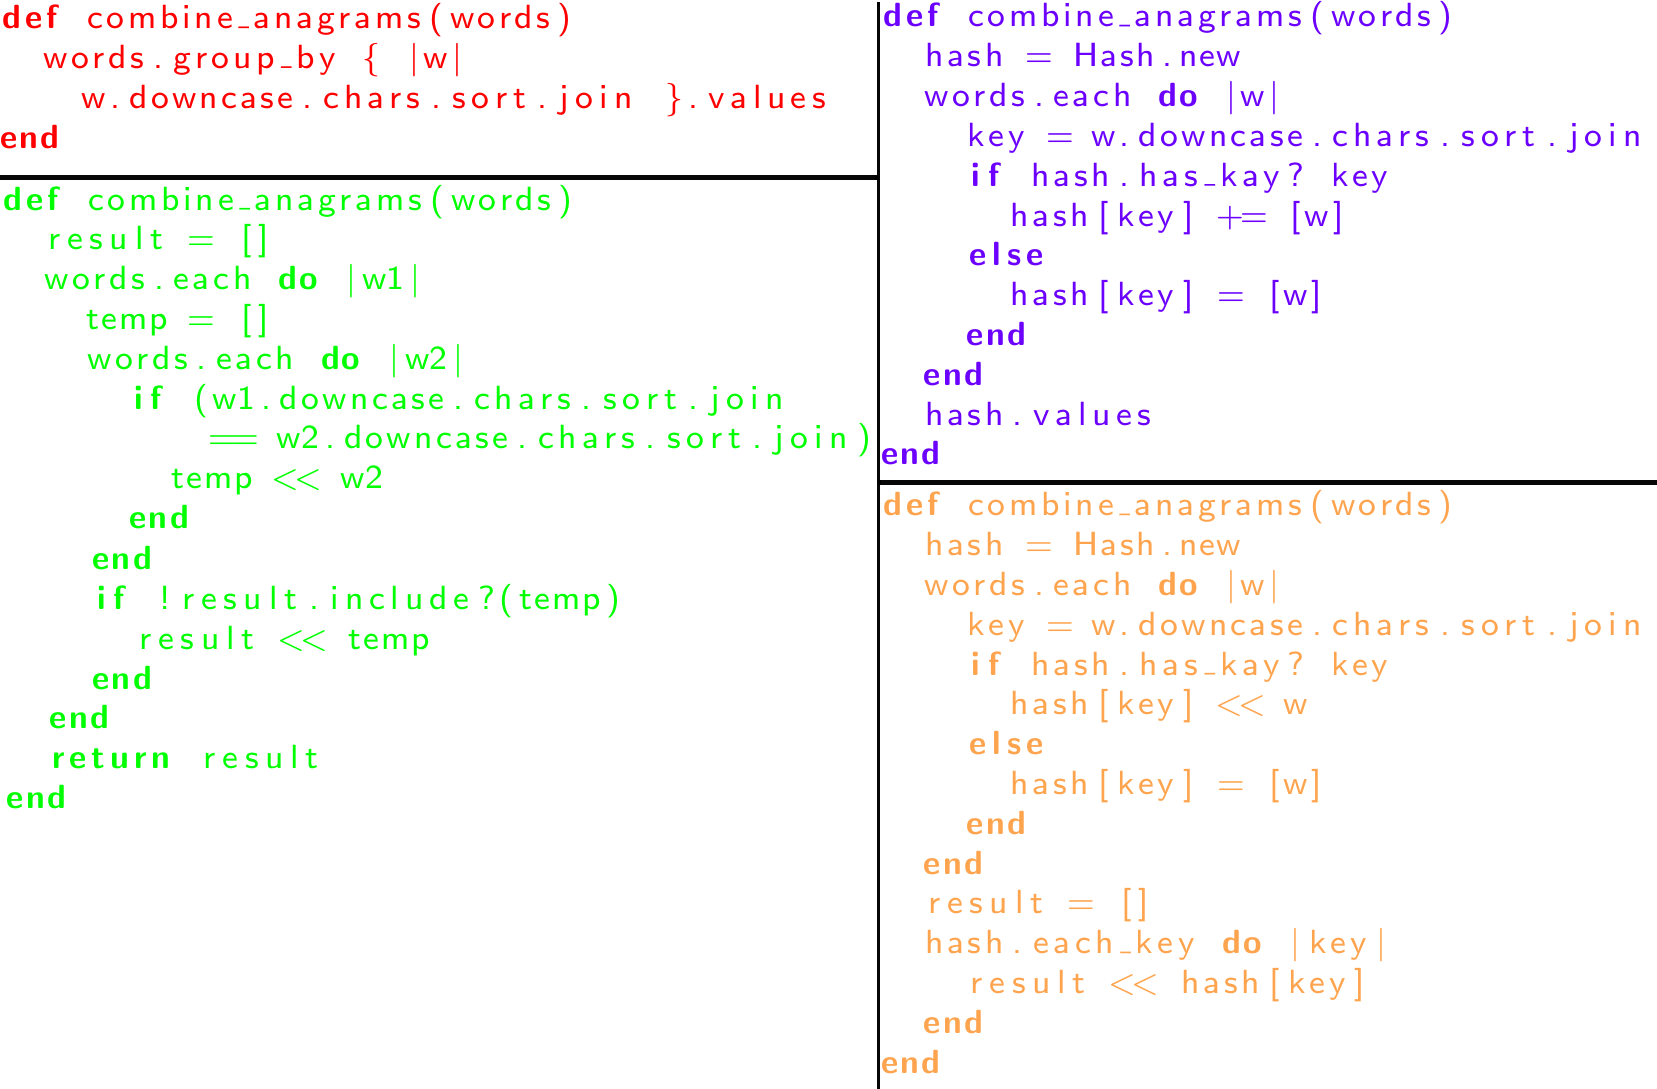
\includegraphics[width=0.7\linewidth]{imagem/implementacoesYin}
		\caption[Quatro implementações distintas que formaram os agrupamentos]{Quatro implementações distintas que formaram os agrupamentos \cite{Yin:2015}}
		\label{fig:implementacoesYin}
		\end{figure}

		\begin{figure}[ht]
			\centering
			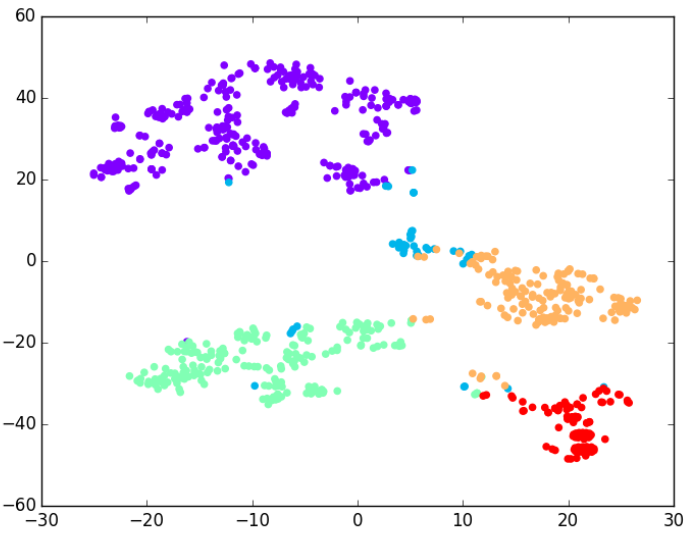
\includegraphics[scale=0.5]{imagem/visualizacao-tSNE.png}
			\caption[Visualização da técnica de projeção t-SNE]{Visualização da técnica de projeção t-SNE \cite{Yin:2015}}
			\label{fig:t-SNE}
		\end{figure}

		Na \cref{fig:t-SNE} é possível observar cinco grupos distintos criados a
		partir da comparação das \acs{TED}s normalizadas destacados em cores diferentes.
		Tais cores foram obtidas, conforme o foco do trabalho para geração e fornecimento
		de dados, para representar os diversos valores obtidos pela métrica ABC
		\cite{fitzpatrick1997applying}, no qual seu tamanho é computado contando o
		número de atribuições, a quantidade de ramos da árvore e as instruções de
		condição para um segmento do código-fonte. Contudo, a finalidade desse projeto é
		o fornecimento de dicas, o qual não é um tópico desta pesquisa. Cada ponto
		presente na visualização corresponde a uma implementação. Todas as
		implementações possuem a função \foreign{combine\_anagrams} que possui a
		variável \foreign{words} como parâmetro (\cref{fig:implementacoesYin}). A
		implementação em vermelho obteve a menor métrica pela utilização de somente
		uma instrução. Os códigos-fontes roxo e laranja obtiveram pontuação semelhante,
		entretanto, esse obteve uma pontuação maior devido a um laço de repetição para
		cada chave presente na \foreign{hash} antes de terminar a função. Por fim, a
		implementação verde obteve a maior pontuação, visto que utilizou de mais instruções
		para resolver o problema. Enquanto os pontos azuis não obtiveram similaridade
		suficiente para formar um agrupamento ou serem classificados em outro agrupamento,
		ou seja, \foreign{outliers}.

		A extração de características por meio da \acs{AST} é interessante, como também
		o uso da \acs{TED} normalizada para verificar sua similaridade, devido ao seu
		baixo custo computacional. Entretanto, como o autor testou seu agrupamento
		somente com implementações para resolver um único problema, não sabemos se
		tal abordagem é eficiente quando houver implementações que buscam resolver
		diversos problemas, em razão da possibilidade dos códigos-fontes gerarem
		árvores parecidas ainda quando solucionam problemas distintos.
		
		Em \citeonline{Glassman:2014}, foi proposto um agrupamento hierárquico de dois
		níveis. No nível mais alto ocorre o agrupamento das soluções, utilizando o
		\foreign{K-means} com diversos valores para $k$, ao longo do plano de separação,
		considerando apenas características abstratas, como, por exemplo: posição da
		declaração de condicional em relação a declarações de laço de repetição (antes,
		dentro ou depois), profundidade de um laço de repetição (\foreign{loop})
		aninhado, números de nós \acs{AST} e declarações de retorno, \foreign{loops} e
		comparações.
		
		Dentro de cada agrupamento de alto nível, é utilizado o \foreign{K-means}
		novamente, para produzir subagrupamentos destinados a capturar a dimensão
		generalizada, construções de linguagem de baixo nível e bibliotecas utilizadas.
		Os agrupamentos internos são formados por meio de 48 características concretas:
		operações aritméticas e lógicas, laços de repetição, funções de bibliotecas,
		declarações de atribuição, \foreign{loops}, condicional, número de variáveis
		e valores constantes, por exemplo.
		
		A validação dos agrupamentos ocorreu por meio da comparação dos \foreign{clusters}
		criados pelo algoritmo de agrupamento com os que foram criados pelos professores.
		Para os professores foram entregues 50 códigos dos estudantes randomicamente
		distribuídos e notou-se que eles ignoraram características de baixo nível.
		Esses autores utilizaram a métrica Informação Mútua Ajustada (\ac{AMI}), cálculo
		probabilístico, para comparar cada agrupamento dos professores com os
		\foreign{clusters} gerado pelo \foreign{k-means} \cite{macqueen1967}. Quando o
		valor de \acs{AMI} é 0 (zero), quer dizer que os agrupamentos são independentes,
		entretanto, se for igual a 1, indica perfeita concordância entre os
		\foreign{clusters}. Quando $k$ tinha um valor maior ou igual a 15, os
		agrupamentos concordaram com o agrupamento de cada professor, conforme medição
		do \acs{AMI}.
		
		Apesar da grande quantidade de dados extraídos das implementações, não houve
		nenhum alusão sobre como essas características interfeririam no cálculo de
		similaridade utilizada. Contudo, a abordagem de dividir as informações a serem
		coletadas em duas dimensões é relevante. Posto que as implementações com
		a mesma quantidade de laços de repetição, por exemplo, deveriam ser agrupadas
		facilitando a verificação se os alunos entenderam como fazer e utilizar
		tal instrução.
		
		Em \citeonline{Taherkhani:2012}, desenvolveu-se uma ferramenta,denominada Aari,
		para classificar implementações baseado na utilização de conjuntos de treinamento
		e teste. Com isso, é necessário o conhecimento prévio de implementações dos
		problemas propostos para treinar o classificador e as características para
		reconhecer as submissões dos alunos. Os autores separaram as características
		em quatro categorias: características numéricas, características descritivas,
		características de algoritmos de ordenação e outras características.
		
%		Em \citeonline{Taherkhani:2012}, testou-se a ferramenta Aari para cinco tipos
%		de métodos de ordenação: \foreign{bubble sort}, \foreign{insertion sort},
%		\foreign{selection sort}, \foreign{mergesort} e \foreign{quicksort}. Os autores
%		separaram as características em quatro categorias: características numéricas,
%		características descritivas, características de algoritmos de ordenação e
%		outras características.
		
		A categoria de características numéricas extrai tudo que pode ser medido
		como inteiro e possui o seguinte conjunto de características: número de
		declarações de atribuição; número de linhas de código; complexidade McCabe;
		total de operadores; total de operandos; número de operadores único; número
		de operando único; total do número de operadores e operandos; total do número
		de operadores e operandos únicos; número de variáveis; número de laços de
		repetição; número de laços aninhados e número de bloco.
		
		A categoria de características descritivas possui: se um algoritmo é
		recursivo, se é uma recursão em cauda, papeis (\foreign{roles}) de variáveis
		e \foreign{arrays}. Essas características podem ser identificadas como booleano,
		indicando ausência ou existência das características correspondentes. Enquanto
		outras características possui informações sobre blocos e laços de repetição,
		informação do contador do \foreign{loop} e informações de dependência.
		
		Após extrair as características, cada algoritmo pode ser representado pelo seu
		vetor de características. A ferramenta do estudo utiliza a técnica de árvore
		de decisão para classificar os algoritmos. É por meio dessa abordagem que os
		autores classificaram os programas enviados por um determinado grupo de alunos.
		
		Para verificar a precisão do Aari, foi realizado uma categorização manual.
		Inicialmente foi realizado um agrupamento manual dos algoritmos de ordenação,
		diferenciando-os em duas etapas. A primeira rodada é referente a implementação
		do algoritmo sem o ensino prévio dos métodos de ordenação descritos
		anteriormente. Desta forma, foi pedido para que 112 alunos implementassem o
		método de ordenação que eles sabiam. Na segunda rodada, foi apresentado
		o funcionamento de cada algoritmo previamente e, após a apresentação, eles
		poderiam implementar qualquer outro algoritmo como também programar o mesmo
		da primeira etapa. Somente 80 alunos participaram da segunda rodada. Esses
		alunos também tinham participado da primeira etapa.
		
		A \cref{fig:clusterManual} apresenta o gráfico do agrupamento manual
		dos métodos de ordenação, \foreign{bubble sort}, \foreign{insertion sort},
		\foreign{selection sort}, \foreign{merge sort} e \foreign{quick sort},
		selecionados para verificar a precisão do Aari. O eixo $x$ é representado
		pelos algoritmos de ordenação citados anteriormente, além da
		\foreign{Inneficiente variations}. Essa última representação é consequência
		de modificações realizadas pelos alunos na estrutura de qualquer algoritmo de
		ordenação. A categoria \foreign{Others} foi criada a partir das implementações
		de outros métodos de ordenação: \foreign{shell sort} e \foreign{heapsort}. O
		eixo $y$ indica a quantidade de implementações reconhecidas. Para cada algoritmo
		de ordenação há duas colunas: a coluna da esquerda representa as soluções
		computacionais da primeira etapa, enquanto a coluna da direita demonstra as
		implementações da segunda rodada. É possível notar, após a apresentação dos
		algoritmos de ordenação na etapa 2, que: poucas implementações foram classificadas
		como \foreign{Inneficiente variations}; menos estudantes optaram em implementar o
		\foreign{bubble sort}, o \foreign{selection sort} e \foreign{Others}; e houve
		mais implementações do \foreign{merge sort} e do \foreign{quick sort}.
		
		\begin{figure}[h]
			\centering
			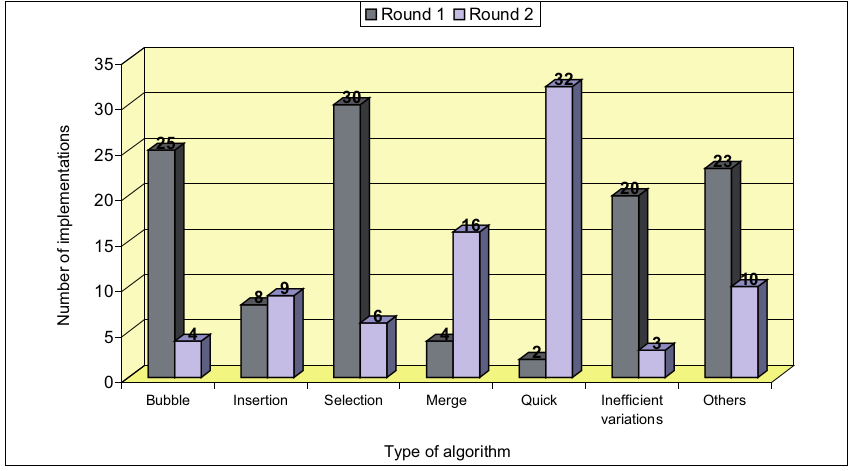
\includegraphics[scale=0.4]{imagem/clusterManual.png}
			\caption[Agrupamento manual das implementações dos estudos estudantes na
			primeira e segunda etapa]{Agrupamento manual das implementações dos estudos estudantes na
			primeira e segunda etapa \cite{Taherkhani:2012}.}
			\label{fig:clusterManual}
		\end{figure}
		
		Após o agrupamento manual dos métodos de ordenação implementados pelos alunos,
		\citeonline{Taherkhani:2012} realizaram o reconhecimento automático das
		implementações por meio da ferramenta Aari utilizando mais uma categoria de
		características, características de algoritmos de ordenação. Tal categoria
		considera as variáveis mais utilizadas, o uso de variáveis temporárias, se o
		algoritmo necessita de uma memória extra. Caso existam dois \foreign{loops}
		aninhados, pode ocorrer dois tipos de características: o laço externo incrementa
		e o laço interno decrementa; e quando o laço interno é inicializado com o valor
		do laço externo. Inicialmente a ferramenta foi treinada para reconhecer os
		algoritmos de ordenação citados anteriormente. A \cref{fig:clusterAutomatico}
		apresenta um gráfico para comparar cada agrupamento manual realizado anteriormente
		com o reconhecimento automático da ferramenta. Possui as mesmas propriedades da
		\cref{fig:clusterManual} com exceção das colunas: a coluna da esquerda referencia
		o agrupamento manual de cada algoritmo de ordenação da segunda etapa e a coluna
		da direita apresenta os algoritmos reconhecidos corretamente pelo Aari. Nota-se
		que todas as implementações dos métodos de ordenação \foreign{bubble sort},
		\foreign{selection sort} e \foreign{quicksort} foram classificados corretamente.
		É possível verificar também que a ferramenta não foi capaz de reconhecer vários
		algoritmos como \foreign{others}, visto que ele não foi treinado para
		reconhecer tais algoritmos.
		
		\begin{figure}[ht]
			\centering
			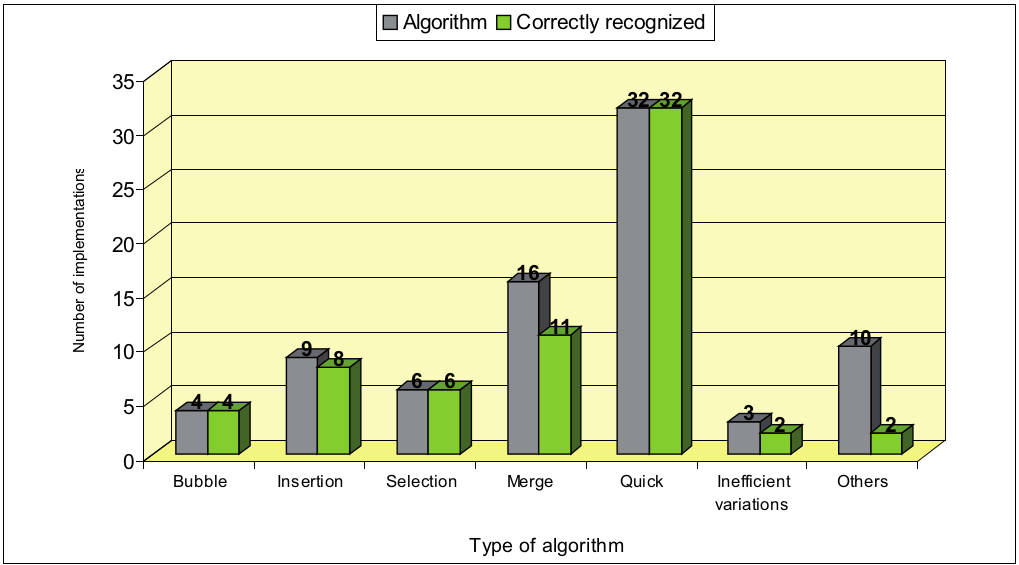
\includegraphics[scale=0.33]{imagem/clusterAutomatico.png}
			\caption[Comparação das implementações dos alunos dos \foreign{clusters}
			manual e automático da segunda etapa]{Comparação das implementações dos alunos dos \foreign{clusters}
			manual e automático da segunda etapa \cite{Taherkhani:2012}.}
			\label{fig:clusterAutomatico}
		\end{figure}
		
		A ferramenta mostrou-se capaz de identificar a maioria dos métodos de ordenação
		para quais foi treinada previamente. Tal abordagem torna-se interessante quando
		há um plano de ensino detalhando os problemas a serem resolvidos, possibilitando
		o treinamento da ferramenta. Entretanto, caso seja utilizado para classificar
		diversos problemas desconhecidos para o classificador, não há uma categorização
		prévia adequada. Desta forma, inviabilizaria sua utilização em \acs{MOOC} se fosse
		utilizado para classificar os problemas de todos os cursos de programação.
		
		\citeonline{Glassman:2015} apresentam uma ferramenta para visualização de
		implementações que apresenta os agrupamentos de códigos-fontes formados,
		fornecendo as principais instruções utilizadas pelas implementações presentes
		em um determinado conjunto de submissões com a finalidade de auxiliar os
		professores que realizarão as correções.
		
%		\citeonline{Glassman:2015} apresentam o OverCode, ferramenta de visualização
%		de informação que mostra os \foreign{clusters} formados, as principais
%		instruções utilizadas pelas implementações presentes em um determinado
%		agrupamento e as linhas de código de uma determinada função/método. A
%		ferramenta é voltada para aqueles que realizarão a correção das submissões.
		
		Para verificar a similaridade das submissões a fim de realizar o agrupamento,
		são realizados os seguintes passos: formatar o código-fonte, executar casos
		de teste, extrair a sequência de variáveis, identificar variáveis em comum,
		renomear variáveis comuns e únicas para, então, realizar o agrupamento.
		Formatar o código-fonte consiste na reformatação de cada implementação: na
		remoção dos espaços entre os \foreign{tokens} (mantendo os espaços somente
		após as palavras reservadas) de comentários e de linhas em branco. Essas
		modificação no código-fonte, além de deixá-lo legível, também permite cada
		linha de código ser representada como uma \foreign{string} para que seja
		possível encontrá-la em outras soluções \cite{Glassman:2015}.
		
		A segunda etapa do agrupamento consiste na execução do mesmo caso de teste
		para todas as implementações. A cada passo da execução, os nomes e valores de
		variáveis locais e globais, bem como o valor de retorno da função são gravados
		como se fosse um histórico de execução ou \foreign{trace}. A partir desse
		histórico, a ferramenta extrai a sequência de valores de todas as variáveis.
		
		A partir do conhecimento da sequência de valores de cada variável, a ferramenta
		identifica quais são as variáveis comuns. Tais variáveis são reconhecidas a
		partir das suas sequências idênticas dado dois ou mais históricos de execução.
		As variáveis que só ocorrem uma vez no \foreign{trace} são as variáveis únicas.
		Após reconhecer as variáveis comuns e únicas, a ferramenta as renomeia para o
		nome da variável que ocorreu em mais históricos de execução.
		
		Após todos esses passos, a normalização do código-fonte realizada em todas as
		implementações garante que o estilo de escrita do aluno não influenciará na
		verificação de similaridade. O agrupamento é realizado por meio da comparação
		estática entre conjuntos de linhas de diversas implementações. Desta forma, não
		utiliza uma técnica de agrupamento e de similaridade específica. Cada agrupamento,
		representado como conjunto de programas, pode possuir 1 ou mais programas cujo
		conjunto de linhas é idêntico.
		
		\begin{figure}[ht]
			\centering
			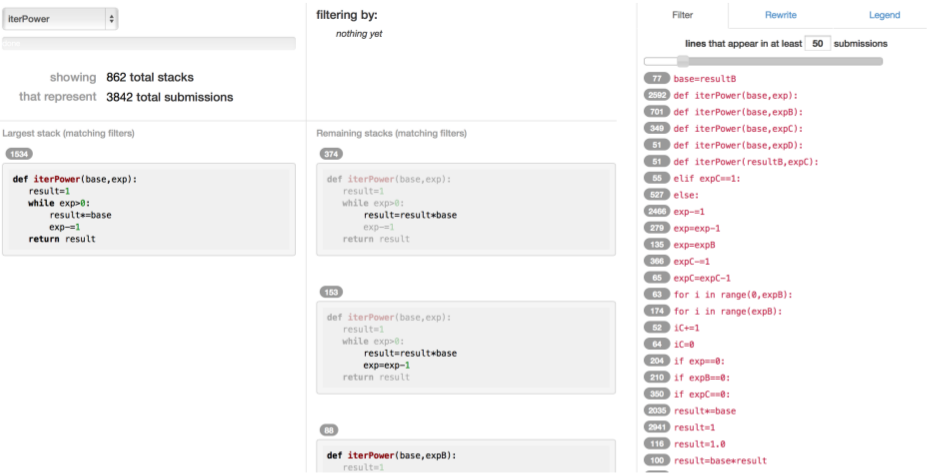
\includegraphics[scale=0.4]{imagem/overCode.png}
			\caption[Interface da ferramenta OverCode]{Interface da ferramenta OverCode \cite{Glassman:2015}.}
			\label{fig:interfaceOverCode}
		\end{figure}
		
		Na \cref{fig:interfaceOverCode}, que exibe a interface da ferramenta proposta,
		o OverCode, é possível notar a utilização do conjunto de programas para
		representar os agrupamentos. A primeira coluna da esquerda exibe dois painéis.
		O primeiro painel apresenta o número de agrupamentos, representado pelos conjuntos de programas,
		e o número total de submissões, enquanto o segundo painel, mostra o maior
		conjunto de programas. A coluna central apresenta a opção de busca, filtrando
		por uma determinada palavra no quadro superior, e as conjunto de programas remanescentes no
		quadro inferior. A terceira coluna apresenta a frequência com que as linhas
		de códigos estão presentes nas soluções dos agrupamentos.

		A comparação dos conjuntos de programas menores com a conjunto de programa maior
		ocorre entre a primeira e a segunda coluna dando ênfase nas linhas que estão
		implementadas diferentes. Com isso, é possível verificar como cada conjunto
		foi montado e a característica daquele agrupamento quando comparada com o
		conjunto maior. Como utiliza análise dinâmica, extraindo o histórico de execução
		para agrupar as submissões, é possível verificar o \foreign{trace} de uma
		variável ao longo de sua execução em um caso de teste a fim de auxiliar os
		usuários a entenderem a execução do algoritmo.
		
		\begin{figure}[h]
			\centering
			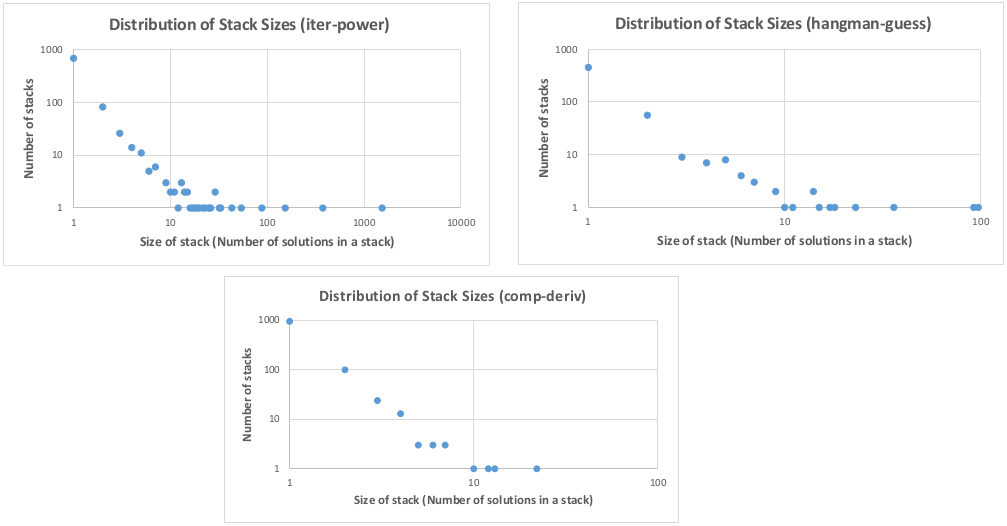
\includegraphics[width=1\linewidth]{imagem/OverCodeDistri}
			\caption[Representação do tamanho dos agrupamentos (conjunto de programas) para cada problema]
			{Representação do tamanho dos agrupamentos (conjunto de programas) para cada problema
				\cite{Glassman:2015}}
			\label{fig:OverCodeDistri}
		\end{figure}

		A \cref{fig:OverCodeDistri} apresenta o agrupamento, representado pela quantidade de
		conjunto de programas no eixo $y$ e o total de submissões em uma conjunto de programa no eixo $x$,  em relação a
		três problemas resolvidos em Python: o problema \texttt{iterPower} refere-se a
		implementação de uma função, que possui a base e o expoente como parâmetros, para
		calcular o exponencial com sucessivas multiplicações; o problema \texttt{hangman}
		possui um vetor de caracteres (\foreign{string}) e uma lista de caractere como
		parâmetros, na qual deve retornas todos os caracteres da \foreign{string} que não
		estão presentes na lista de caracteres; por fim, o problema \texttt{compDeriv}
		calcula a derivada de um polinomial, no qual os coeficientes estão presentes em
		uma lista. Esses problemas obtiveram 3875, 1118 e 1433 soluções corretas submetidas,
		respectivamente. Na devida ordem, a maior conjunto de programa de cada problema são constituídas
		de 1534, 97 e 22 implementações e 684, 452 e 959 conjuntos de programas com apenas uma solução.

		Por fim, os autores concluíram que a interface auxilia os professores a terem
		uma visão de alto nível das soluções (implementações), podendo compreender os
		erros e fornecer um \foreign{feedback} mais relevante, devido ao agrupamento
		das implementações. Isso diminui consideravelmente a quantidade de submissões
		a serem efetivamente corrigidas.
		
		A análise dinâmica e os recursos realizados para que fosse montado a conjunto de programa
		mostrou-se eficiente, principalmente para o problema \texttt{iterPower}, no
		qual sua maior conjunto de programa obteve quase 40\% das implementações corretas. Com isso,
		torna-se evidente o quanto a ferramenta pode auxiliar os professores a realizar
		as correções dos códigos-fontes. A etapa de padronização do código realizado
		durante a análise, no qual verifica-se as variáveis comuns e renomeia-as,
		contribui com a comparação bloco a bloco, devido a partes do bloco, onde
		ocorrem a utilização dessas variáveis, serem parecidas. Poderia ter sido
		verificado todos os problemas implementados em apenas um código-fonte para
		verificar qual seria o resultado dos agrupamentos e compará-los.
		
		\citeonline{Wei2015} apresentam uma ferramenta para auxiliar na correção das
		submissões do \acs{MOOC} de forma a agrupar pedaços (\foreign{chuncks}) de códigos
		fontes semelhantes, agrupá-los conforme sua similaridade e alocar cada conjunto
		de implementações ao estudante com conhecimento suficiente para revisá-los.
		
		O particionamento do código tem por objetivo torná-lo legível e fácil de
		compreender para a correção. A ferramenta realiza o particionamento por funções.
		Também foi necessário normalizar cada submissão a fim de encontrar o estilo de
		escrita, visto que até mesmo o nome da variável pode alterar o estilo de escrita.
		A ferramenta desenvolvida por \citeonline{Wei2015} normaliza o código por meio
		de três regras: remoção de espaços, linhas em branco e comentários; exclusão
		de palavras reservadas da linguagem de programação, identificadores predefinidos
		e nomes de funções de bibliotecas; e substituição dos identificadores de
		variáveis do usuário por um símbolo especial.
		
		Com isso foi calculado um valor \foreign{hash} para todas as \foreign{k-substring}
		de um código-fonte, sendo $k$ a quantidade de \foreign{substrings} da implementação,
		a fim de verificar a similaridade do estilo de escrita \foreign{token} a
		\foreign{token} é utilizado o algoritmo de \texttt{winnowing} \cite{schleimer2003}
		para escolher o menor subconjunto do estilo de escrita a fim de realizar as
		comparações por meio do coeficiente de similaridade de \foreign{Jaccard} \cite{jaccard1901}.
		
		E com a finalidade de identificar a dificuldade da implementação, foi utilizado
		a distância Euclidiana para comparar as características extraídas -- quantidade
		de métodos invocados e laços de repetição aninhados -- e o \ac{k-NN} para identificar
		o nível de dificuldade de revisão do \foreign{chunck}.
		
		\begin{figure}
			\centering
			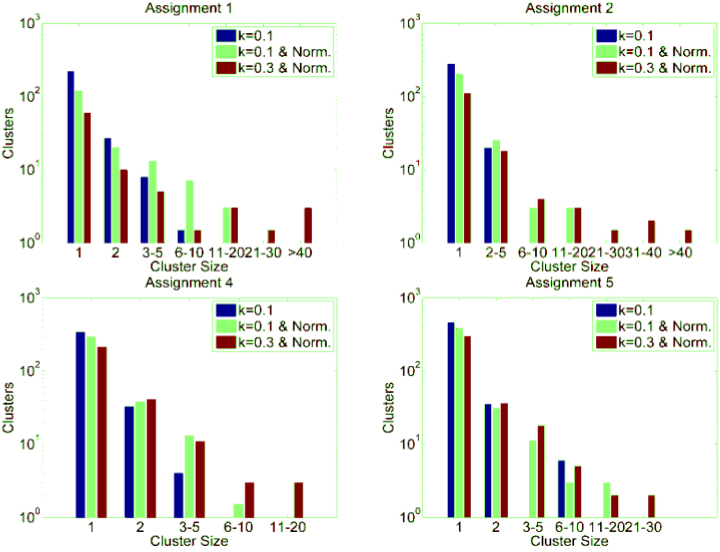
\includegraphics[width=0.7\linewidth]{imagem/clusteringPerformance}
			\caption[Distribuição dos agrupamentos]{Distribuição dos agrupamentos \cite{Wei2015}.}
			\label{fig:clusteringPerformance}
		\end{figure}
		
		A \cref{fig:clusteringPerformance} apresenta a distribuição dos
		agrupamentos em quatro problemas distintos. Para todos os gráficos, a
		abcissa é referente ao tamanho dos pedaços, enquanto a ordenada representa
		o número de agrupamentos. É possível notar três tipos de agrupamento. A barra
		horizontal azul representa o agrupamento sem normalização. Enquanto as barras
		verde e vermelho possuem o valor de $k$ diferente, entretanto ambas estão
		normalizadas. As tarefas 1 e 2 possuem apenas uma função para resolver um
		pequeno problema e apresentou bons agrupamentos, nos quais possuíam mais
		de 40 implementações em um mesmo grupo quando $k$ era igual a 0,3. As
		tarefas 4 e 5 possuem implementações com várias funções, por esse motivo,
		os agrupamentos não foram satisfeitos, principalmente quando não normalizados.
		Por fim, pode-se notar que a distribuição dos \foreign{chuncks} sem normalização
		de código é inadequado, visto que vários pedaços em todas as tarefas estavam
		sozinhos, e o maior agrupamento possuía entre 6 a 10 funções.
		
		É possível notar que a abordagem dos códigos-fontes compostas de diversas
		funções (tarefas 4 e 5) não obteve sucesso, pois, independente da tarefa
		selecionada, nota-se que a maioria dos \foreign{clusters} formados possuíam
		apenas um código-fonte. Entretanto, a submissão de implementações contendo
		apenas uma função (tarefas 1 e 2) para resolver o problema torna-se interessante,
		devido à realização de alguns agrupamentos com mais de 40 implementações
		semelhantes. Em um ambiente controlado, no qual todos os alunos irão submeter
		diversas soluções com somente uma função, é interessante a utilização da
		ferramenta. Caso contrário, seu uso não interferirá significativamente no
		auxílio a correções de códigos-fontes. 
		
		% TODO: revisar tabela e deixar mais sucinta as colunas 3 (características extraídas), 5 (avaliação) e 6 (conclusões).
			\begin{table}[h]
				\tiny
				\begin{tabularx}{\linewidth}{ |X|X|X|X|X|X|X| }
					\hline % Primeira linha
					\textbf{Artigos}
					& \textbf{Dados de entrada}
					& \textbf{Característica extraídas dos dados de entrada}
					& \textbf{Algoritmo para cálculo de distância ou similaridade}
					& \textbf{Algoritmo de clusterização / Classificador}
					& \textbf{Avaliação}
					& \textbf{Conclusões} \\
					\hline % Segunda Linha
					\citeonline{Yin:2015,Moghadam:2015:ATC,choudhury2016autostyle}
					& Implementações
					& Árvore de sintaxe abstrata
					& Distância de Edição de \acs{TED} normalizada que utiliza estrutura
					\foreign{top-down} e pontuação silhueta
					& \acs{OPTICS}
					& Agrupamento de algoritmos baseado nas soluções de um problema.
					Em cada \foreign{cluster}, identifica as diferenças nas
					implementações de uma abordagem particular
					& \acs{TED} normalizado demonstra conjuntos mais estáveis e menos discrepantes \\
					\hline % Terceira linha
					\citeonline{Glassman:2014}
					& Implementações
					& 12 características de alto nível dos elementos da linguagem e
					instruções relacionados com laços de repetição. 48 características
					de baixo nível envolvendo operações primitivas.
%					& Linguagem de alto nível: 12 características - posição de declarações
%					condicionais em relação a instruções de \foreign{loop}, profundidade
%					dos \foreign{loops} aninhados, números de nós AST, instruções de
%					retorno, laços, comparações, etc. Linguagem de baixo nível: 48
%					características - operações aritméticas, comparações, \foreign{loops},
%					funções de bibliotecas, declarações, número de variáveis do programa,
%					valores constantes, etc.
					& Informação Mútua Ajustada
					& K-means
					& Utilizando a métrica \acs{AMI}, compara os agrupamento automatizados com
					os manuais. 0 indica agrupamentos puramente independentes e 1, perfeita
					concordância entre os agrupamentos.
					& Para k maior ou igual a 15, encontrou-se alta concordância entre os
					\foreign{cluster} do k-means e do professor \\
					\hline % Quarta linha
					\citeonline{Taherkhani:2012}
					& Implementações
					& Características extraídas com valores inteiros, específicas de
					métodos de ordenação, do contador de \foreign{loops} e dependência
					de informação e para reconhecer padrões para classificação.
%					& As características numéricas são extraídas com valores inteiros.
%					As descritivas são específicas de métodos de ordenação. As de algoritmos
%					de ordenação são informações do contador de \foreign{loops}
%					e dependência de informação. E as outras características são para
%					reconhecer padrões para classificação.
					& Vetor de características,calculada a partir das características extraídas
					das implementações
					& C4.5 (árvore de decisão)
					& Comparação da ferramenta com a classificação manual dos professores.
					& Bons resultados para algoritmos de ordenação que foram utilizados na
					fase de treinamento. E taxa de acerto considerável baseado em um possível
					erro do professor. \\
					\hline % Quinta linha
					\citeonline{Glassman:2015,glassman2016clustering,glassman2014interacting,glassman2013toward,glassman2013visualizing}
					& Implementações
					& Rastro do programa e blocos de código.
					& Diferença entre o tamanho dos conjuntos de linhas
					& Comparação entre conjuntos de linhas de código
					& Grande quantidade de conjunto de programas com poucos blocos de código-fonte e poucas
					conjunto de programas com grande quantidade de blocos implementados
					& Possibilidade de retornar um \foreign{feedback} mais preciso para cada
					grupo e facilita a observação da solução do problema. \\
					\hline % Sexta linha
					\citeonline{Wei2015}
					& Implementações
					& Normaliza o código e considera apenas o estilo de escrita do estudante
					& Coeficiente de similaridade de Jaccard
					& Algoritmo \foreign{Winnowing}
					& Classificação de \foreign{workload}: distância Euclidiana e \acs{k-NN}
					& A agrupamento por pedaços de código aumentou sua eficiência. \\
					\hline
				\end{tabularx}
				\caption{Principais informações dos trabalhos relacionados}
				\label{tab:caracPrinc}
			\end{table}
		
		A \cref{tab:caracPrinc} apresenta as principais características de cada trabalho
		relacionado importantes para o desenvolvimento desse projeto. Possibilitando a
		comparação dos tipos de análises utilizados, quais características foram
		extraídas a partir dessas análises e qual abordagem obteve melhor desempenho.
		
		Ambas as abordagens que utilizaram pedaços das implementações para realizar
		o agrupamento \cite{Glassman:2015,Wei2015} mostraram-se vantajosos pela
		quantidade de conjuntos de linhas ou \foreign{chunks} agrupados. A renomeação
		de variáveis comuns, obtidas por meio de casos de teste, também é interessante
		devido ao fato de igualar as instruções que utilizam tais variáveis a fim de
		realizar as comparações \cite{Glassman:2015}. Apesar da utilização das \acs{AST}s
		somente em um único problema \cite{Yin:2015}, tal abordagem obteve agrupamentos
		significativos a fim de auxiliar os professores para realizar as correções.
		
		Contudo, a utilização de um algoritmo de classificação para identificar
		implementações semelhantes \cite{Taherkhani:2012} torna-se inviável a utilização
		da ferramenta em \acs{MOOC} que contenha diversos tipos de problema, devido a necessidade
		de realizar o conjunto de treinamento e teste a fim de treinar o classificador.
		E a abordagem utilizando dois níveis hierárquicos para agrupamento \cite{Glassman:2014}   % TODO: explicar melhor o raciocínio: não temos implementações a priori e não existe garantia que essas implementações, caso existam, sejam representativas de todas as possíveis implementações de algoritmos para a resolução de um problema. Na seção sobre características de programas, precisamos incluir um diagrama mostrando a relação entre problemas, algoritmos e implementações, deixando evidente a questão e subsidiando a resposta aqui.
		possui um conjunto de características vasto, mas a maioria das características pode
		ser descartada no momento do agrupamento manual realizado pelos professores.
		Isso pode ter ocorrido pelo fato dos códigos-fontes utilizados na pesquisa não
		representarem todas as soluções possíveis de um problema. Não é possível afirmar
		isso, visto que não possuímos as implementações.
